\documentclass[10pt]{article}
\usepackage[portuguese]{babel}
\usepackage[utf8]{inputenc}
\usepackage{color}
\usepackage{enumitem}
\usepackage{float}
\usepackage{graphicx}
\usepackage{minted}
\usepackage{geometry}
\geometry{%
    a4paper,
    total={150mm,257mm},
}
\usepackage{hyperref}
\hypersetup{%
    colorlinks=true,
    linkcolor=blue,
    filecolor=magenta,
    urlcolor=cyan,
}

\setlength{\arrayrulewidth}{0.3mm}
\setlength{\tabcolsep}{10pt}
% \setlength{\parindent}{0em}
\renewcommand{\arraystretch}{1.5}
% \renewcommand{\thesection}{}
% \renewcommand{\thesubsection}{}
% \renewcommand{\thesubsubsection}{}

\begin{document}
\begin{center}
    {\scshape Instituto Superior Técnico\par}
    \vspace{1cm}
    {\scshape\Large Applications and Computation for the Internet of Things\par}
    \vspace{1.5cm}
\end{center}
{\scshape\LARGE 2\textsuperscript{st} Lab Work: Sensing the Physical World}
\\
\begin{table}[h!]
    \centering
    \begin{tabular}{|l|l|p{10cm}|}
        \hline
        \multicolumn{3}{|l|}{Group: 12} \\[1.5ex] \hline
        Student 1 & 98380 & Dominika Florczykowska \\ [1.5ex]\hline
        Student 2 & 97144 & Pedro Mendes \\ [1.5ex]\hline
    \end{tabular}
\end{table}

\section{Goal:}
The goal of this work is to sense physical quantities and to control actuators
according to the measured environment.

\section{Description:}
Build an embedded system using an Arduino UNO board to simultaneously control 3
LEDs (the actuators) depending on the state of 3 different sensors –
temperature, rotation angle (potentiometer) and light intensity.

\begin{itemize}
    \item Temperature --- The yellow LED associated with the temperature sensor
        must be turned on when the temperature read is greater than 26 oC (value
        to be eventually redefined at the laboratory according to the
        environment conditions).
    \item Rotation --- The green LED controlled by the potentiometer must blink
        with a period of time varying continuously between 0.2 and 2 seconds,
        depending of the rotation angle applied to the potentiometer.
    \item Light --- The red LED for the light intensity function must change
        continuously its own light intensity based on the light intensity sensed
        in the surrounding environment from
        \begin{list}{$\circ$}{}
            \item Darkness $\rightarrow$ LED fully ON, to
            \item Brightness $\rightarrow$ LED OFF
        \end{list}
\end{itemize}

A diagram of the circuit is represented in the figure.

\begin{figure}[H]
    \centering
    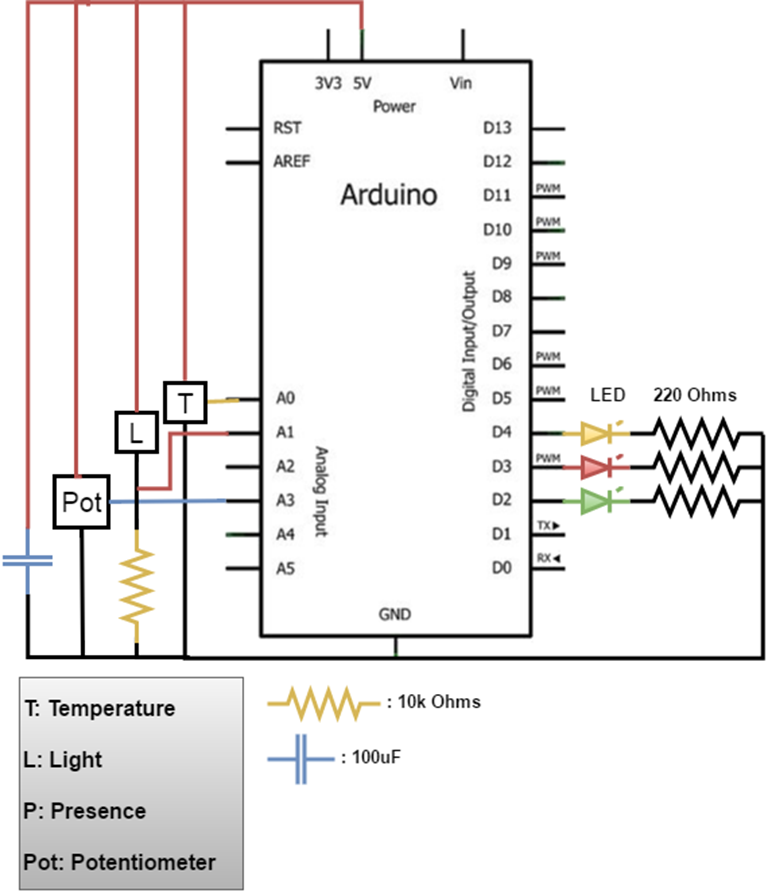
\includegraphics[width=\textwidth]{arduino.png}
\end{figure}

\section{References}

\begin{enumerate}
    \item \url{https://www.arduino.cc/en/Reference/digitalWrite}
    \item \url{https://www.arduino.cc/en/Reference/AnalogRead}
    \item \url{https://www.arduino.cc/en/Reference/Serial}
    \item \url{https://www.arduino.cc/en/Tutorial/Calibration}
    \item \url{https://www.arduino.cc/en/Tutorial/PWM}
    \item \url{https://www.arduino.cc/en/Reference/Delay}
\end{enumerate}

\section{Mapping analog measurements}\label{s:mapping}

Usually the digital readings retrieved from sensors do not correspond directly
to the value of the physical quantity, but rather to values between 0 and a
maximum binary value (such as, for a 10 bits word, $1023 = 210 - 1$). Therefore
some mapping may be required.

When the value is relative just to an offset a simple mapping is adequate, but
in general a more complex scale conversion will be needed. The map function,
available in the Arduino IDE, simplifies these types of conversions. For
example, when rotating a Servo motor with input from a potentiometer we know
that when the value of the potentiometer is 0 then the servo angle must be 0° as
well. Logically, if the value of the potentiometer is 1023 (its maximum reading)
then the servo angle must be 180° (its maximum position):

\[map(value, 0, 1023, 0, 180)\]

Besides this some sensors require a linearization of its transfer function
(physical quantity $\rightarrow$ electrical quantity, such as voltage). For
example, to convert the reading from a circuit with a temperature sensor (in our
case a temperature dependent resistor) to the real temperature several
transformations may be required

\begin{itemize}
    \item to linearize the transfer function of the sensing device $RT = f(T)$, and
    \item to linearize the transfer function of the circuit in which the sensor
        is included.
\end{itemize}

For the device and configuration to be used (based on a TMP35 component) check the function
\[T = (((sensor value / 1024.0) \times 5.0) - 0.5) \times  100\]

\section{Programming with analog sensors:}
To access an external analog sensor you must attach it to an Arduino analog pin. The software allocation of a sensor to an analog pin is done using the following code:

\begin{minted}{cpp}
    int const tempSensor = A0;
\end{minted}

Where \texttt{A0} is the physical pin where the sensor is attached.

To read the value assigned to a specific pin use the Arduino function
\texttt{analogRead(PIN)}, as follows:

\begin{minted}{cpp}
    int temperatureValue = analogRead(tempSensor);
\end{minted}

\section{Debug:}
In order to control some variables and debug your program it is possible to print them to the Serial Monitor available in the Arduino IDE. This kind of tool is useful, for example, to keep track of the temperature variation or to help the calibration of the system.

To use this feature, first start a serial communication with the PC:

\begin{minted}{cpp}
    void setup() { ...; Serial.begin(9600); ...; }
\end{minted}

Then, just \texttt{Serial.print} your variables and/or strings:
\begin{minted}{cpp}
    Serial.println(temperatureValue);
\end{minted}



\section{Program the application:}


Structure the program modularly clearly segmenting the program in separate code
blocks, one for each function to be implemented (e.g.\ read temperature sensor,
control temperature alarm).  In the next laboratory work you will have to
distribute several functions across separate Arduino controllers.

Avoid, or use very carefully, the delay function provided in the Arduino IDE since it just stops the execution flow during the specified time interval.

\subsection{Code:}

\subsubsection{File: \texttt{sensor.hpp}}

\inputminted{arduino}{../sensor.hpp}

\subsubsection{File: \texttt{lab2.ino}}
\inputminted{arduino}{../lab2.ino}

\subsection{Questions:}

\paragraph{Question:}

For each of the three pairs sensor-actuator describe:

\begin{enumerate}
    \item the mapping process implemented;
    \item the calibration setup;
    \item the process, or technique, used to modulate the behaviour of the
        actuator;
    \item the setup prepared to demonstrate the functionality of the system.
\end{enumerate}

\paragraph{Answer:}

The Arduino has an \texttt{analogRead} range from 0 to 1023, and an
\texttt{analogWrite} range from 0 to 255, therefore the data from any analogRead
needs to be mapped to fit into the smaller range.

\begin{itemize}
    \item \textbf{Temperature:}
        This sensor's value had to be linearized as explained in
        Section~\ref{s:mapping}. Using the function described there,
        \[T = (((sensor value / 1024.0) \times 5.0) - 0.5) \times  100\]
        we where able to obtain the temperature in degrees.

        To demonstrate the functionality simply touch the sensor with both
        fingers to increase the temperature above 25 degrees, this constant was
        picked for being above room temperature, but low enough that body heat
        can be enough to light up the LED.
    \item \textbf{Light:}
        To calibrate the sensor 2 experiments were performed to obtain the 2
        extremes, first the sensor was placed in a dark room with an opaque piece
        of plastic on top of it to obtain the lowest possible reading, which was
        `1`, then the sensor was exposed to a bright white light (phone
        flash light) to obtains the highest possible reading which was 1021.

        These values were then mapped to the accepted range of the
        \texttt{analogWrite} function $[0, 255]$. This interval is actually
        inverted when passed to the map function since the LED will light up at
        its highest intensity when the sensor reads lowest level of light in the
        environment.

        \[map(value, 1, 1021, 255, 0)\]

        The modulation of the behaviour is just a direct call to
        \texttt{analogWrite} with the value returned from \texttt{map}.
    \item \textbf{Rotation:}
        The calibration of this sensor was simple, we measured the value read
        from \texttt{analogRead} when it was at the minimum and maximum
        rotation, these mapped exactly to 0 and 1023. Since we work in
        milliseconds, we then map this range to the range $[200, 2000]$ (0.2
        seconds to 2 seconds) which will be stored as the current blink period
        (in the code named \texttt{blink\_period}).

        Then to modulate the behaviour of the actuator, the program checks the
        \texttt{millis} function and the last time the led state has been
        changed, and sees if \texttt{blink\_period} has passed, if so, then the
        led state is toggled.
\end{itemize}

\paragraph{Question:}

What is the system software pattern of the application?

\paragraph{Answer:}

Round Robin pattern. All the tasks are executed continuously in the main loop in
the same order (one at a time). Each task checks for the value read by a
corresponding sensor and responds by showing correct output with the use of LED.
%% This could use a better explanation, maybe read the slides and
% copy from there

\paragraph{Question:}

What are the timing constraints of the system?

\paragraph{Answer:}

%% idk what he means

\end{document}
